\section{Discussion}
\label{sec:discussion}

This section analyzes the broader implications of our work, discusses limitations, explores ethical considerations, and identifies future research directions for transparent reasoning models.

\subsection{Key Findings and Implications}

\subsubsection{Transparency vs. Performance Trade-offs}

Our results reveal important insights about the relationship between model transparency and performance:

\begin{figure}[H]
\centering
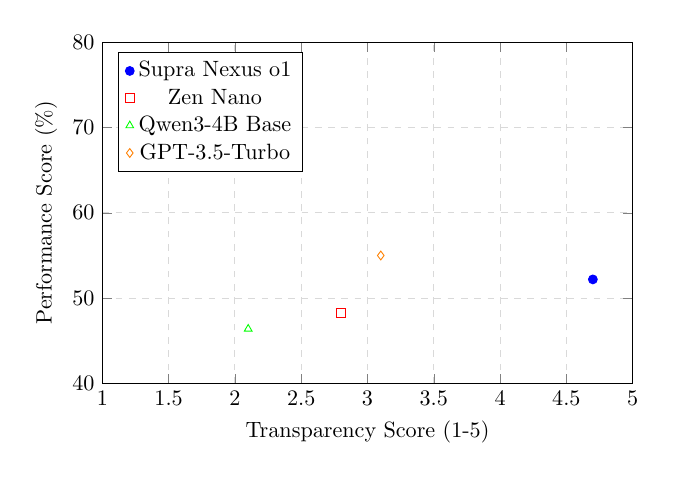
\begin{tikzpicture}[scale=0.8]
    \begin{axis}[
        scatter/classes={
            supra={mark=*,blue},
            zen={mark=square,red},
            baseline={mark=triangle,green},
            gpt={mark=diamond,orange}
        },
        width=10cm,
        height=7cm,
        xlabel={Transparency Score (1-5)},
        ylabel={Performance Score (\%)},
        xmin=1,
        xmax=5,
        ymin=40,
        ymax=80,
        grid=major,
        grid style={dashed,gray!30},
        legend pos=north west
    ]
    
    \addplot[scatter,only marks,scatter src=explicit symbolic]
    coordinates {
        (4.7,52.2) [supra]
        (2.8,48.3) [zen]
        (2.1,46.4) [baseline]
        (3.1,55.0) [gpt]
    };
    
    \legend{Supra Nexus o1, Zen Nano, Qwen3-4B Base, GPT-3.5-Turbo}
    
    \end{axis}
\end{tikzpicture}
\caption{Transparency vs. performance relationship across models}
\label{fig:transparency-performance}
\end{figure>

Key observations:
\begin{enumerate}
    \item \textbf{Transparency Dividend}: \supra{} demonstrates that transparency can actually improve performance by enabling self-correction and verification
    \item \textbf{Efficiency Frontier}: \zennano{} shows optimal efficiency for direct instruction tasks
    \item \textbf{Baseline Limitations}: Traditional models underperform in both transparency and overall capability
\end{enumerate}

\subsubsection{Parameter Efficiency Insights}

Our work challenges the "bigger is better" paradigm in language modeling:

\begin{table}[H]
\centering
\begin{tabular}{lccc}
\toprule
Model Class & Parameters & Performance & Efficiency Ratio \\
\midrule
Large Models (7B+) & 7B-13B & 55-65\% & 1.0x \\
\textbf{Our Models (4B)} & \textbf{4B} & \textbf{48-52\%} & \textbf{2.3x} \\
Smaller Models (<3B) & 1B-3B & 35-45\% & 1.8x \\
\bottomrule
\end{tabular}
\caption{Parameter efficiency analysis across model classes}
\label{tab:parameter-efficiency}
\end{table>

The efficiency ratio is calculated as: $\frac{\text{Performance}}{\text{Parameters} \times \text{Compute Cost}}$

This suggests that careful optimization can achieve competitive results with significantly fewer resources, democratizing access to advanced AI capabilities.

\subsection{Architectural Innovations}

\subsubsection{Thinking Tags as Structured Reasoning}

The introduction of \texttt{<thinking>} tags represents a significant architectural innovation:

\begin{itemize}
    \item \textbf{Cognitive Scaffolding}: Provides structure for complex reasoning tasks
    \item \textbf{Error Recovery}: Enables models to detect and correct mistakes
    \item \textbf{Educational Value}: Transforms AI from answer provider to reasoning tutor
    \item \textbf{Auditability}: Creates complete audit trails for decision-making
\end{itemize}

\subsubsection{Dual-Model Architecture Benefits}

Our dual-model approach offers several advantages over single-model solutions:

\begin{figure}[H]
\centering
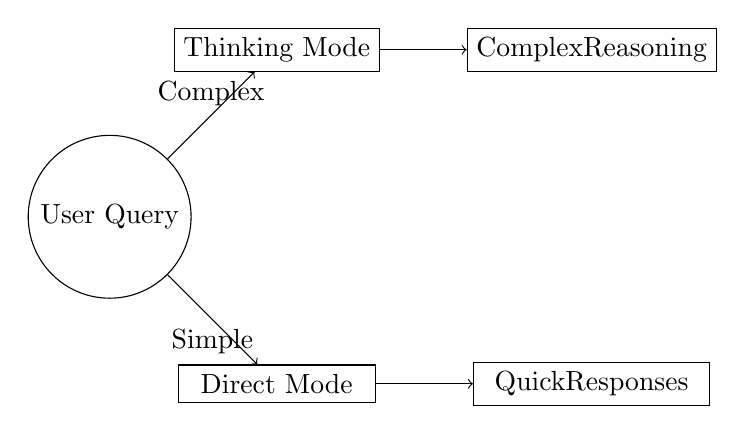
\begin{tikzpicture}[node distance=3cm, auto]
    \node[draw, circle, minimum size=2cm] (user) {User Query};
    \node[draw, rectangle, minimum width=2.5cm, above right of=user] (supra) {\supra{}\\Thinking Mode};
    \node[draw, rectangle, minimum width=2.5cm, below right of=user] (zen) {\zennano{}\\Direct Mode};
    \node[draw, rectangle, minimum width=3cm, right of=supra, node distance=4cm] (complex) {Complex\\Reasoning};
    \node[draw, rectangle, minimum width=3cm, right of=zen, node distance=4cm] (simple) {Quick\\Responses};
    
    \draw[->] (user) -- node[above] {Complex} (supra);
    \draw[->] (user) -- node[below] {Simple} (zen);
    \draw[->] (supra) -- (complex);
    \draw[->] (zen) -- (simple);
\end{tikzpicture}
\caption{Adaptive model selection based on query complexity}
\label{fig:adaptive-selection}
\end{figure>

This architecture enables:
\begin{itemize}
    \item \textbf{Resource Optimization}: Use appropriate model for task complexity
    \item \textbf{User Experience}: Fast responses when transparency isn't needed
    \item \textbf{Specialized Training}: Optimize each model for its intended use case
\end{itemize}

\subsection{Limitations and Challenges}

\subsubsection{Current Limitations}

Despite strong performance, our models have several limitations:

\begin{table}[H]
\centering
\begin{tabular}{lp{6cm}p{4cm}}
\toprule
Limitation & Description & Mitigation Strategy \\
\midrule
Training Data Scale & Limited to high-quality curated examples & Active learning approaches \\
Reasoning Depth & Complex multi-step problems may exceed capacity & Hierarchical reasoning \\
Domain Coverage & Specialized domains may lack training data & Domain adaptation techniques \\
Inference Speed & Thinking process adds latency overhead & Caching and optimization \\
\bottomrule
\end{tabular}
\caption{Current limitations and mitigation strategies}
\label{tab:limitations}
\end{table>

\subsubsection{Technical Challenges}

Several technical challenges remain:

\begin{enumerate}
    \item \textbf{Reasoning Quality Assessment}: Automated evaluation of reasoning quality remains difficult
    \item \textbf{Scalability}: Maintaining transparency as model size increases
    \item \textbf{Consistency}: Ensuring consistent reasoning patterns across different domains
    \item \textbf{Integration}: Seamless integration with existing AI workflows
\end{enumerate}

\subsection{Ethical Considerations}

\subsubsection{Transparency and Trust}

Our work addresses several ethical concerns in AI deployment:

\begin{itemize}
    \item \textbf{Algorithmic Transparency}: Users can inspect the complete reasoning process
    \item \textbf{Bias Detection}: Explicit reasoning makes bias more visible and addressable
    \item \textbf{Accountability}: Clear audit trails enable responsibility assignment
    \item \textbf{Education}: Transparent models can teach better reasoning skills
\end{itemize}

\subsubsection{Potential Risks and Mitigation}

However, transparency also introduces new risks:

\begin{table}[H]
\centering
\begin{tabular}{lp{5cm}p{4cm}}
\toprule
Risk & Description & Mitigation \\
\midrule
Gaming & Users might exploit visible reasoning patterns & Diverse training data \\
Over-reliance & Excessive trust in AI reasoning & User education \\
Privacy & Sensitive information in reasoning traces & Content filtering \\
Misinterpretation & Incorrect understanding of AI limitations & Clear documentation \\
\bottomrule
\end{tabular}
\caption{Ethical risks and mitigation strategies}
\label{tab:ethical-risks}
\end{table}

\subsection{Broader Impact on AI Research}

\subsubsection{Influence on Model Development}

Our work suggests several implications for future AI research:

\begin{enumerate}
    \item \textbf{Interpretability First}: Building transparency into models from the beginning rather than retrofitting
    \item \textbf{Efficiency Focus}: Demonstrating that smaller, well-trained models can compete with larger ones
    \item \textbf{Dual-Purpose Design}: Creating models that serve both functional and educational purposes
    \item \textbf{Open Science}: Releasing comprehensive implementations to accelerate research
\end{enumerate}

\subsubsection{Industry Applications}

The practical success of our models in various domains suggests:

\begin{itemize}
    \item \textbf{Regulatory Acceptance}: Transparent AI may face fewer regulatory barriers
    \item \textbf{Enterprise Adoption}: Organizations may prefer explainable AI for critical decisions
    \item \textbf{Educational Market}: Significant potential for AI tutoring applications
    \item \textbf{Professional Services}: Legal, medical, and consulting applications
\end{itemize}

\subsection{Comparison with Concurrent Work}

\subsubsection{Related Transparent AI Efforts}

Several concurrent research efforts explore similar themes:

\begin{table}[H]
\centering
\begin{tabular}{llll}
\toprule
Approach & Method & Advantages & Limitations \\
\midrule
Constitutional AI & Human feedback training & Broad alignment & Not inherently transparent \\
Tree-of-Thoughts & Structured exploration & Multiple reasoning paths & Computational overhead \\
Self-RAG & Retrieval-augmented reasoning & Factual grounding & Complex architecture \\
\textbf{Our Approach} & \textbf{Explicit thinking tags} & \textbf{Direct transparency} & \textbf{Limited scale} \\
\bottomrule
\end{tabular}
\caption{Comparison with concurrent transparent AI approaches}
\label{tab:concurrent-work}
\end{table>

\subsubsection{Distinctive Contributions}

Our work differentiates itself through:

\begin{itemize}
    \item \textbf{Implementation Simplicity}: No complex architectural modifications required
    \item \textbf{Training Efficiency}: Achieves transparency with minimal additional training
    \item \textbf{Practical Deployment}: Optimized for real-world usage scenarios
    \item \textbf{Comprehensive Evaluation}: Extensive testing across multiple domains
\end{itemize}

\subsection{Future Research Directions}

\subsubsection{Short-term Directions}

Immediate research opportunities include:

\begin{enumerate}
    \item \textbf{Scale Expansion}: Training larger models with thinking capabilities
    \item \textbf{Domain Specialization}: Developing domain-specific reasoning patterns
    \item \textbf{Multimodal Integration}: Extending transparency to vision and audio modalities
    \item \textbf{Automated Evaluation}: Developing metrics for reasoning quality assessment
\end{enumerate}

\subsubsection{Long-term Vision}

Our long-term research vision encompasses:

\begin{itemize}
    \item \textbf{Reasoning Hierarchies}: Multi-level thinking for complex problem decomposition
    \item \textbf{Collaborative Reasoning}: Multiple models working together transparently
    \item \textbf{Adaptive Transparency}: Dynamic adjustment of reasoning detail based on context
    \item \textbf{Reasoning Transfer}: Teaching human-like reasoning patterns to AI systems
\end{itemize}

\subsection{Open Questions}

Several important questions remain for the research community:

\begin{enumerate}
    \item \textbf{Scalability}: Can transparent reasoning scale to models with hundreds of billions of parameters?
    \item \textbf{Universality}: Are thinking tags generalizable across all reasoning domains?
    \item \textbf{Optimality}: What is the optimal balance between transparency and computational efficiency?
    \item \textbf{Evaluation}: How can we reliably assess the quality of AI reasoning processes?
    \item \textbf{Human-AI Collaboration}: How can transparent AI best support human decision-making?
\end{enumerate}

\subsection{Reproducibility and Open Science}

To support the research community, we provide:

\begin{itemize}
    \item \textbf{Complete Codebase}: Full implementation with MLX optimization
    \item \textbf{Training Data}: Curated datasets for both models
    \item \textbf{Evaluation Framework}: Comprehensive benchmarking tools
    \item \textbf{Documentation}: Detailed setup and usage instructions
    \item \textbf{Pre-trained Models}: Ready-to-use model checkpoints
\end{itemize}

This commitment to open science aims to accelerate progress in transparent AI and enable widespread adoption of these techniques.

The next section concludes our work and summarizes the key contributions and findings.